\section{Generación y puesta en marcha de la base de datos}

Ha llegado el momento de ponernos manos a la masa y dejarnos de preparativos o presentación de herramientas. Vamos a levantar nuestra base de datos.
\\El diagrama final de la base de datos quedaría como podemos ver en la figura \ref{fig:db-design}.
\begin{figure}
    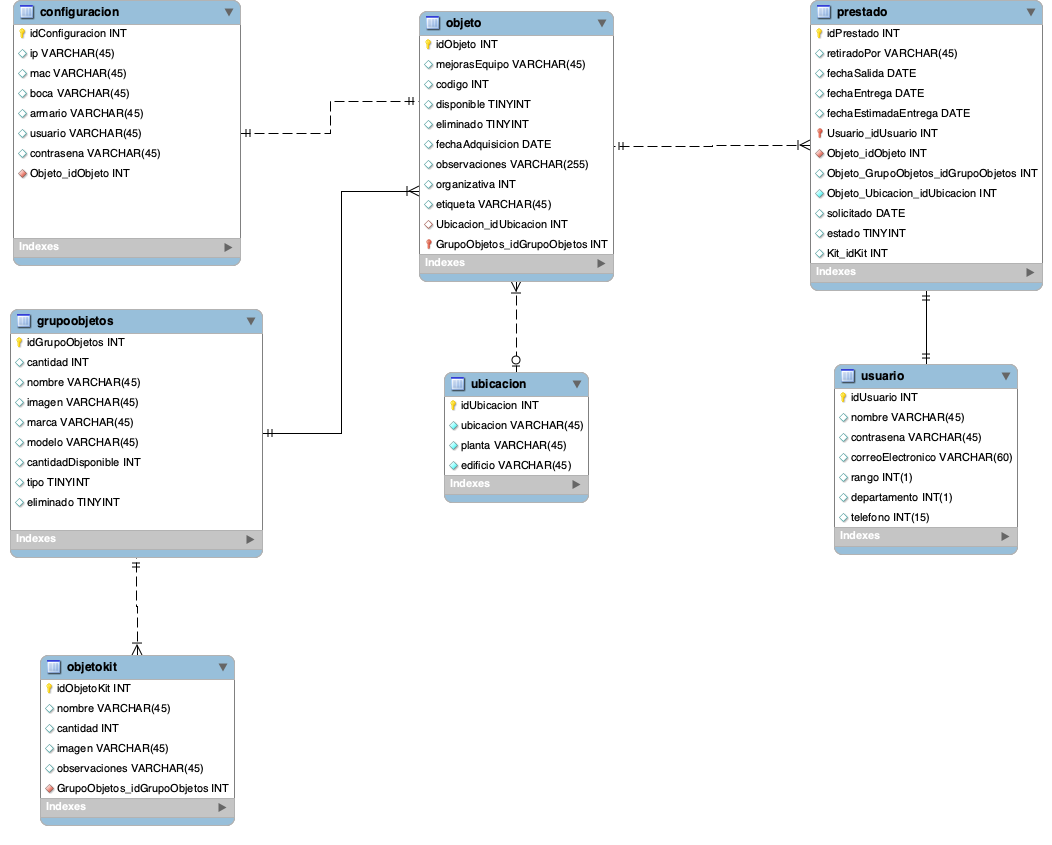
\includegraphics[width=\textwidth,height=\textheight,keepaspectratio]{db_design.png}
    \caption{Diseño final de la base de datos}\label{fig:db-design}
\end{figure}
Generamos el script ``.sql'' para poder generar nuestra base de datos.
\\Esta configuración la basaremos únicamente en la sección de código que añadiremos a nuestro archivo docker-compose.yml para poder hacerlo.
\\Añadimos la versión que utilizaremos de docker-compose:

\begin{verbatim}
version: "3.9"
\end{verbatim}

Creamos el apartado ``services'':

\begin{verbatim}
    services:
\end{verbatim}

Y añadimos nuestro primer contenedor, el de la base de datos:

\begin{verbatim}
    db:
    container_name: inventarium_sql
    image: mariadb:10.7.1-focal
    ports:
      - "3306:3306"
    volumes:
      - ./dump:/docker-entrypoint-initdb.d
      - persistent:/var/lib/mysql
    networks:
      - default
    environment:
      MYSQL_DATABASE: ualinventarium
      MYSQL_USER: ualinventarium
      MYSQL_PASSWORD: contraseñasecreta
      MYSQL_ROOT_PASSWORD: contraseñasecreta
\end{verbatim}
\begin{itemize}
    \item \textbf{db}: Este es el nombre que le hemos puesto como referencia para docker-compose.
    \item \textbf{container\_name}: Es el nombre que tendrá el contenedor que vayamos a desplegar.
    \item \textbf{image}: La imagen utilizada, es decir, la ``máquina virtual'' que vamos a levantar. En este caso es una máquina virtual de MariaDB.
    \item \textbf{ports}: Los puertos que utilizará la máquina, a la izquierda son los que le llegan a la máquina y a la derecha los que salen.
    \item \textbf{volumes}: Esta sección es muy importante ya que aquí podremos importar archivos en el momento del despliegue de nuestro entorno. En este caso estamos importando la carpeta ``dump'' donde dentro está el archivo de generación de la base de datos. También le enlazamos el volumen ``persistent'' que creamos más adelante. Esto es para que no perdamos datos cuando paremos el contenedor. Ya que los datos de la base de datos de esta se almacenará en un sitio externo.
    \item \textbf{networks}: Aquí podemos añadir las redes que manejará nuestro contenedor. En este caso es la default.
    \item \textbf{environment}: Dentro de environments podremos definir variables que se necesiten en el momento del despliegue de nuestro contenedor. En este caso definimos el nombre de la base de datos, el usuario junto a su contraseña y la contraseña del usuario root.
\end{itemize}
\begin{verbatim}
    phpmyadmin:
    container_name: inventarium_php_adm
    image: phpmyadmin:5.1
    links:
      - db:db
    ports:
      - 8000:80
    environment:
      MYSQL_USER: user
      MYSQL_PASSWORD: user
      MYSQL_ROOT_PASSWORD: user
    networks:
      - default
\end{verbatim}
Este despliegue es para phpmyadmin, nuestro gestor de base de datos. Como añadido al punto anterior tenemos el apartado \textbf{links} que nos ayuda a crear una vinculación de un contenedor con otro. En este caso le estamos pasando la información de nuestra base de datos para que trabaje sobre ella.
\begin{verbatim}
volumes:
    persistent: {}
\end{verbatim}
Dentro de la sección \textbf{volumes} podemos generar volúmenes que se van a utilizar dentro de nuestros contenedores. En este caso hemos creado nuestro volumen ``persistent'' para poder guardar la información que se almacene dentro de nuestra base de datos.
\vspace{\baselineskip}
\\Para levantar nuestra base de datos ejecutaríamos dentro del directorio donde hemos creado nuestro docker-compose.yml el siguiente comando:
\begin{verbatim}
    sudo docker compose up
\end{verbatim}
Ya tendríamos nuestra base de datos en funcionamiento.
\vspace{\baselineskip}
\begin{tcolorbox}
    [colback=green!5!white,colframe=green!75!black,fonttitle=\bfseries,title=¿Cómo comprobamos los resultados?]
    Visual Studio Code realiza una \textbf{tunelización de los puertos} a partir de la conexión SSH. Es decir, podemos ir habilitando redireccionamientos de puertos para poder ir viendo los resultados en nuestra máquina. Esto resulta de gran ayuda ya que no hay que realizar una configuración en la máquina de apertura de puertos para poder ir trabajando sobre cada una de las aplicaciones existentes. Ya que el funcionamiento del sistema será interno con poder disponer de los puertos HTTP Y HTTPS abiertos no necesitamos más.
\end{tcolorbox}

